% ============================================================
%  TD N°06 — Support Vector Machines (SVM)
%  Compte Rendu Académique
%  Auteur : Chabbaki Ayman — MDSBDIA26 — Groupe G1
% ============================================================
\documentclass[12pt,a4paper]{article}

% ─── Encodage & Langue ──────────────────────────────────────
\usepackage[utf8]{inputenc}
\usepackage[T1]{fontenc}
\usepackage[french]{babel}

% ─── Mise en page ───────────────────────────────────────────
\usepackage[top=2.5cm, bottom=2.5cm, left=2.5cm, right=2.5cm]{geometry}
\usepackage{fancyhdr}
\usepackage{titlesec}
\usepackage{parskip}
\usepackage{setspace}

% ─── Typo ───────────────────────────────────────────────────
\usepackage{lmodern}
\usepackage{microtype}

% ─── Couleurs & Graphiques ──────────────────────────────────
\usepackage[dvipsnames,table]{xcolor}
\usepackage{graphicx}
\usepackage{float}
\usepackage{subcaption}
\usepackage{tikz}

% ─── Maths ──────────────────────────────────────────────────
\usepackage{amsmath,amssymb,amsthm}
\usepackage{mathtools}
\usepackage{bm}

% ─── Tableaux ───────────────────────────────────────────────
\usepackage{booktabs}
\usepackage{tabularx}
\usepackage{array}
\usepackage{multirow}
\usepackage{colortbl}

% ─── Code ───────────────────────────────────────────────────
\usepackage{listings}
\usepackage{minted}

% ─── Boîtes ─────────────────────────────────────────────────
\usepackage[most]{tcolorbox}
\tcbuselibrary{breakable, skins}

% ─── Liens ──────────────────────────────────────────────────
\usepackage{hyperref}
\hypersetup{colorlinks=true, linkcolor=darkblue, urlcolor=tealcolor}

% ─── Divers ─────────────────────────────────────────────────
\usepackage{enumitem}
\usepackage{xspace}

% ============================================================
%  Palette couleurs
% ============================================================
\definecolor{darkblue}{RGB}{26,37,80}
\definecolor{tealcolor}{RGB}{26,122,110}
\definecolor{crimson}{RGB}{156,61,56}
\definecolor{amber}{RGB}{176,125,58}
\definecolor{lightgray}{RGB}{245,245,245}
\definecolor{midgray}{RGB}{180,180,180}
\definecolor{svmpurple}{RGB}{91,61,143}

% ============================================================
%  Titres
% ============================================================
\titleformat{\section}
  {\large\bfseries\color{darkblue}}
  {\thesection.}{.5em}{}
  [\color{tealcolor}\rule{\linewidth}{0.6pt}]

\titleformat{\subsection}
  {\normalsize\bfseries\color{tealcolor}}
  {\thesubsection}{.5em}{}

\titleformat{\subsubsection}
  {\small\bfseries\color{amber}}
  {\thesubsubsection}{.5em}{}

% ============================================================
%  En-tête / Pied de page
% ============================================================
\pagestyle{fancy}
\fancyhf{}
\fancyhead[L]{\small\color{darkblue}\bfseries TD 6 — Support Vector Machines}
\fancyhead[R]{\small\color{darkblue} Chabbaki Ayman · MDSBDIA26 · G1}
\fancyfoot[C]{\small\color{midgray}--- \thepage\ ---}
\renewcommand{\headrulewidth}{0.4pt}
\renewcommand{\headrule}{\hbox to\headwidth{\color{darkblue}\leaders\hrule height\headrulewidth\hfill}}

% ============================================================
%  Environnements tcolorbox
% ============================================================
\tcbset{
  base/.style={
    breakable, enhanced,
    fonttitle=\bfseries\small,
    left=6pt, right=6pt, top=5pt, bottom=5pt,
    boxrule=0.5pt
  }
}

\newtcolorbox{reponsebox}[1][]{
  base,
  colback=tealcolor!8,
  colframe=tealcolor,
  coltitle=white,
  colbacktitle=tealcolor,
  title={Réponse},
  #1
}

\newtcolorbox{resultbox}[1][]{
  base,
  colback=darkblue!6,
  colframe=darkblue,
  coltitle=white,
  colbacktitle=darkblue,
  title={Résultat expérimental},
  #1
}

\newtcolorbox{observbox}[1][]{
  base,
  colback=amber!8,
  colframe=amber,
  coltitle=white,
  colbacktitle=amber,
  title={Observation clé},
  #1
}

\newtcolorbox{theorbox}[1][]{
  base,
  colback=svmpurple!6,
  colframe=svmpurple,
  coltitle=white,
  colbacktitle=svmpurple,
  title={Théorie SVM},
  #1
}

% ============================================================
%  Style code listings
% ============================================================
\lstset{
  language=Python,
  basicstyle=\ttfamily\scriptsize,
  backgroundcolor=\color{lightgray},
  frame=single,
  rulecolor=\color{midgray},
  breaklines=true,
  keywordstyle=\color{darkblue}\bfseries,
  stringstyle=\color{crimson},
  commentstyle=\color{midgray}\itshape,
  numbers=left,
  numberstyle=\tiny\color{midgray},
  numbersep=5pt,
  showstringspaces=false,
  tabsize=4,
}

% ============================================================
\begin{document}
% ============================================================

% ─── Page de titre ──────────────────────────────────────────
\begin{titlepage}
\begin{tikzpicture}[remember picture, overlay]
  \fill[darkblue] (current page.north west) rectangle
    ([yshift=-4.5cm] current page.north east);
  \fill[tealcolor] ([yshift=-4.5cm] current page.north west) rectangle
    ([yshift=-5.1cm] current page.north east);
  \fill[svmpurple] ([yshift=-5.1cm] current page.north west) rectangle
    ([yshift=-5.4cm] current page.north east);
\end{tikzpicture}

\vspace*{2.5cm}
{\color{white}\raggedright
  \hspace{1cm}{\fontsize{11}{13}\selectfont Master Intelligence Artificielle}\par
  \hspace{1cm}{\fontsize{10}{12}\selectfont Machine Learning — Semestre 2024–2025}\par
  \vspace{0.6cm}
  \hspace{1cm}{\fontsize{9}{11}\selectfont\color{white!80!darkblue}
    Pr. BEN LAHMAR EL Habib}
}

\vspace{3.5cm}
\begin{center}
  \begin{tcolorbox}[
    enhanced, width=0.88\textwidth,
    colback=white, colframe=darkblue,
    boxrule=2pt, arc=4pt,
    drop shadow={darkblue!40}
  ]
    \centering
    \vspace{0.4cm}
    {\color{svmpurple}\fontsize{10}{12}\selectfont\bfseries TRAVAUX DIRIGÉS N°\,06}\\[0.4cm]
    {\color{darkblue}\fontsize{18}{22}\selectfont\bfseries Support Vector Machines}\\[0.2cm]
    {\color{darkblue}\fontsize{14}{17}\selectfont\bfseries (SVM)}\\[0.3cm]
    {\color{tealcolor}\fontsize{10}{12}\selectfont\itshape
      Marge maximale · Kernel trick · GridSearchCV · BankChurners}\\[0.3cm]
    \vspace{0.2cm}
    \color{midgray}\rule{0.7\linewidth}{0.5pt}\\[0.3cm]
    {\fontsize{11}{13}\selectfont\bfseries Chabbaki Ayman}\\[0.1cm]
    {\color{tealcolor}\fontsize{10}{12}\selectfont MDSBDIA26 — Groupe G1}\\[0.3cm]
    \vspace{0.2cm}
  \end{tcolorbox}
\end{center}

\vfill
\begin{center}
\begin{tabular}{ccc}
  \textcolor{darkblue}{\textbf{Dataset}} & \quad & \textcolor{darkblue}{\textbf{Outils}} \\
  \textcolor{tealcolor}{BankChurners · Moons · Circles} & & \textcolor{tealcolor}{sklearn · numpy · matplotlib} \\[1em]
  \textcolor{darkblue}{\textbf{Modèles}} & & \textcolor{darkblue}{\textbf{Date}} \\
  \textcolor{tealcolor}{SVC · SVR · GridSearchCV} & & \textcolor{tealcolor}{Juin 2026}
\end{tabular}
\end{center}
\end{titlepage}

% ─── Table des matières ─────────────────────────────────────
\tableofcontents
\newpage

% ============================================================
\section{Introduction — Les Machines à Vecteurs de Support}
% ============================================================

\begin{theorbox}
Les SVM (Support Vector Machines) cherchent l'\textbf{hyperplan séparateur à marge maximale}. Formellement, pour un problème binaire avec données $\{(\mathbf{x}_i, y_i)\}$, $y_i \in \{-1, +1\}$ :

\textbf{Problème primal (hard margin)} :
\[
\min_{\mathbf{w}, b} \frac{1}{2}\|\mathbf{w}\|^2 \quad \text{s.c.} \quad y_i(\mathbf{w}\cdot\mathbf{x}_i + b) \geq 1 \;\forall i
\]

\textbf{Marge} $= \dfrac{2}{\|\mathbf{w}\|}$ \qquad
\textbf{Soft margin (C)} : $\displaystyle\min_{\mathbf{w},b,\bm{\xi}} \frac{\|\mathbf{w}\|^2}{2} + C\sum_i\xi_i$

\textbf{Kernel trick} : $K(\mathbf{x},\mathbf{y}) = \langle\varphi(\mathbf{x}),\varphi(\mathbf{y})\rangle$ sans calculer $\varphi$ explicitement.
Noyaux : Linéaire $\mathbf{x}^\top\mathbf{y}$, RBF $\exp(-\gamma\|\mathbf{x}-\mathbf{y}\|^2)$, Polynomial $(\gamma\mathbf{x}^\top\mathbf{y}+r)^d$.
\end{theorbox}

Le dataset utilisé tout au long du TD est \textbf{BankChurners} : 10\,127 clients bancaires, 19 variables, taux de churn de \textbf{16,07\%}. Après encodage et split stratifié 80/20 : 8\,101 exemples d'entraînement, 2\,026 en test.

% ============================================================
\section{Partie 1 — SVM Linéaire : Visualisation de la Marge}
% ============================================================

\subsection{Q1.1 — Hard Margin : marge maximale sur données séparables}

\begin{resultbox}
\begin{center}
\begin{tabular}{lccc}
\toprule
\textbf{Modèle} & \textbf{Vecteurs support} & $\|\mathbf{w}\|$ & \textbf{Marge} $= 2/\|\mathbf{w}\|$ \\
\midrule
SVM linéaire (C=1000) & 3 (classe -1: 2, classe +1: 1) & 0.2672 & \textbf{7.486} \\
\bottomrule
\end{tabular}
\end{center}
$\mathbf{w} = [0{,}2005,\; -0{,}1766]$, \quad $b = 0{,}7846$
\end{resultbox}

\begin{figure}[H]
  \centering
  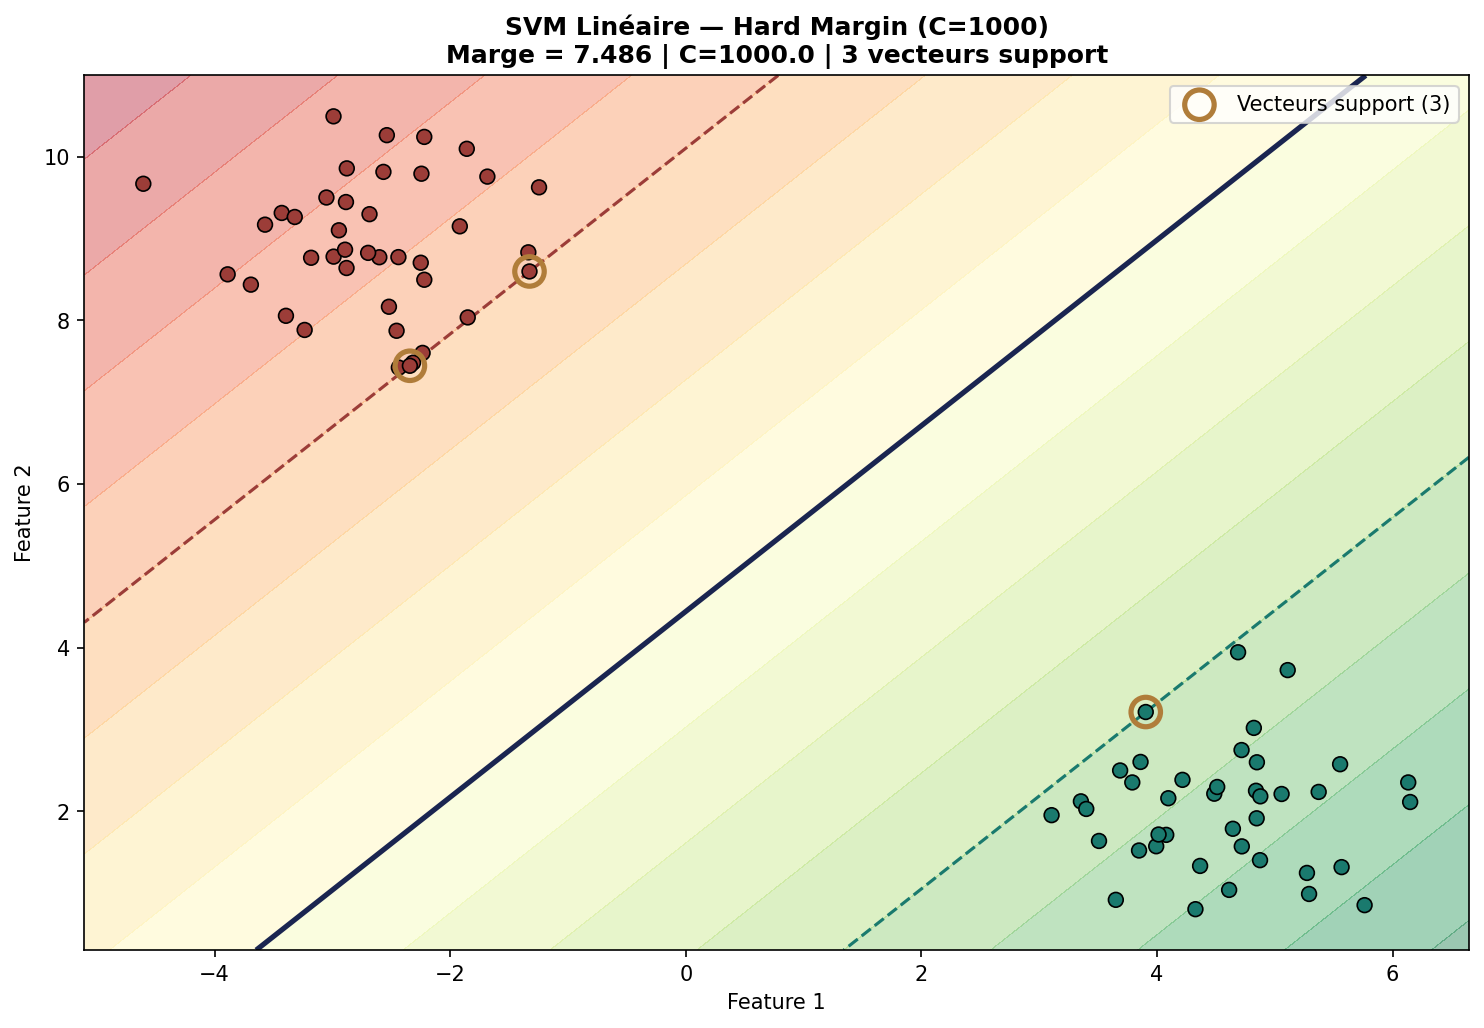
\includegraphics[width=0.82\textwidth]{fig_svm_hard_margin.png}
  \caption{SVM linéaire hard margin (C=1000) — hyperplan (trait plein bleu), hyperplans marginaux (tirets), vecteurs support (cercles oranges). Marge = 7{,}486.}
  \label{fig:hard_margin}
\end{figure}

\begin{reponsebox}
\textbf{Q1 — Nombre de vecteurs support et propriété fondamentale :}

Seuls \textbf{3 exemples} (sur 80) sont des vecteurs support. Ils se trouvent exactement sur les hyperplans marginaux $y_i(\mathbf{w}\cdot\mathbf{x}_i + b) = 1$. La propriété fondamentale : \textbf{la solution SVM ne dépend que des vecteurs support}. En ré-entraînant le SVM sur ces seuls 3 exemples, on obtient des coefficients $\mathbf{w}$ et $b$ \textbf{identiques} (à la précision numérique près). Les 77 autres exemples peuvent être supprimés sans modifier l'hyperplan optimal.

\textbf{Q2 — Calcul de la marge :} $\text{Marge} = \dfrac{2}{\|\mathbf{w}\|} = \dfrac{2}{\sqrt{0{,}2005^2 + 0{,}1766^2}} = \dfrac{2}{0{,}2672} = 7{,}486$. Cette valeur correspond à la distance géométrique entre les deux hyperplans marginaux parallèles.
\end{reponsebox}

\subsection{Q1.2 — Soft Margin : effet du paramètre C}

\begin{resultbox}
\begin{center}
\begin{tabular}{rrrr}
\toprule
$C$ & \textbf{Marge} & \textbf{NB vecteurs support} & \textbf{Régularisation} \\
\midrule
0{,}01  & 5{,}499 & 17 & Forte (biais élevé) \\
0{,}10  & 3{,}983 & 4  & Modérée \\
1{,}00  & 3{,}187 & 3  & Défaut \\
10{,}00 & 3{,}187 & 3  & Faible \\
100{,}00 & 3{,}187 & 3 & Très faible (variance) \\
\bottomrule
\end{tabular}
\end{center}
\end{resultbox}

\begin{figure}[H]
  \centering
  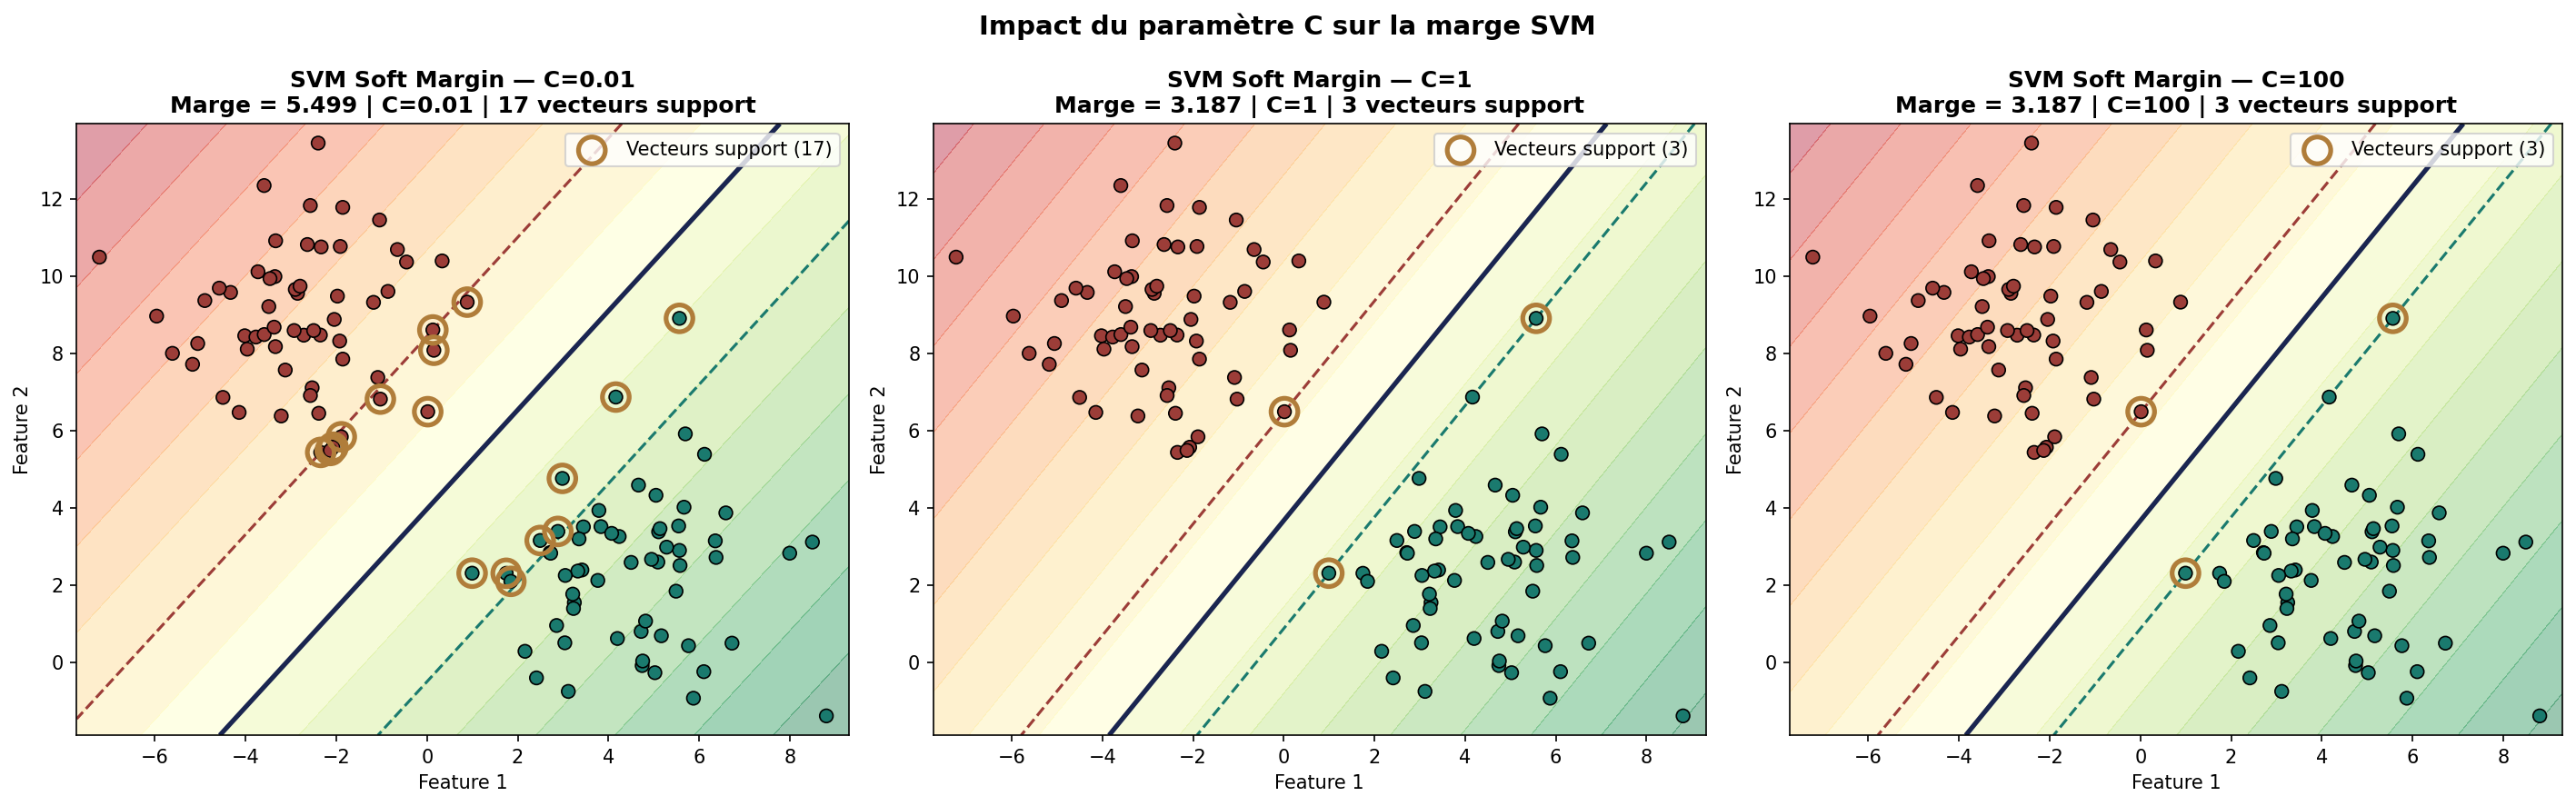
\includegraphics[width=\textwidth]{fig_svm_soft_margin.png}
  \caption{Impact de C sur la marge SVM (données avec chevauchement, cluster\_std=1{,}8). De gauche à droite : C=0{,}01 (marge large, 17 SV), C=1 (équilibre), C=100 (marge étroite, SV réduits).}
  \label{fig:soft_margin}
\end{figure}

\begin{reponsebox}
\textbf{Q4 — Comparaison C=0{,}01 vs C=100 :}

\begin{itemize}[leftmargin=1.5em]
  \item \textbf{C=0{,}01} (régularisation forte) : marge = 5{,}499, 17 vecteurs support. L'algorithme tolère de nombreuses violations ($\xi_i > 0$) pour maximiser la marge. Résultat : frontière plus généraliste mais moins précise.
  \item \textbf{C=100} (régularisation faible) : marge = 3{,}187, 3 vecteurs support. L'algorithme cherche à respecter les contraintes $y_i(\mathbf{w}\cdot\mathbf{x}_i+b) \geq 1$ au maximum → frontière plus précise mais potentiellement sur-ajustée.
\end{itemize}

\textbf{Q5 — Erreurs avec C=1000 ?} Oui. Les données générées avec cluster\_std=1{,}8 ne sont \textbf{pas linéairement séparables} — il existe un chevauchement entre les deux distributions gaussiennes. Un hyperplan linéaire ne peut pas séparer parfaitement ces classes, quel que soit C.

\textbf{Q6 — Dataset bruité — quel C recommander ?} Un C modéré (0{,}1 à 10) offre le meilleur compromis. Analogie : $C = 1/\lambda$ où $\lambda$ est la régularisation L2 de la Régression Logistique. \textbf{Grand C = faible régularisation} dans les deux modèles.
\end{reponsebox}

% ============================================================
\section{Partie 2 — Le Kernel Trick : Séparation Non-Linéaire}
% ============================================================

\subsection{Q2.1 — Comparaison des noyaux sur données Moons}

\begin{resultbox}
\begin{center}
\begin{tabular}{lrrl}
\toprule
\textbf{Noyau} & \textbf{Accuracy test} & \textbf{Vecteurs support} & \textbf{Frontière} \\
\midrule
Linéaire (C=1)      & 0{,}9200 & 77 & Droite (inadaptée) \\
RBF (C=1, scale)    & \textbf{0{,}9467} & 69 & Courbe, épouse les lunes \\
Polynomial (d=3)    & 0{,}9067 & 78 & Courbe polynomiale \\
\bottomrule
\end{tabular}
\end{center}
\end{resultbox}

\begin{figure}[H]
  \centering
  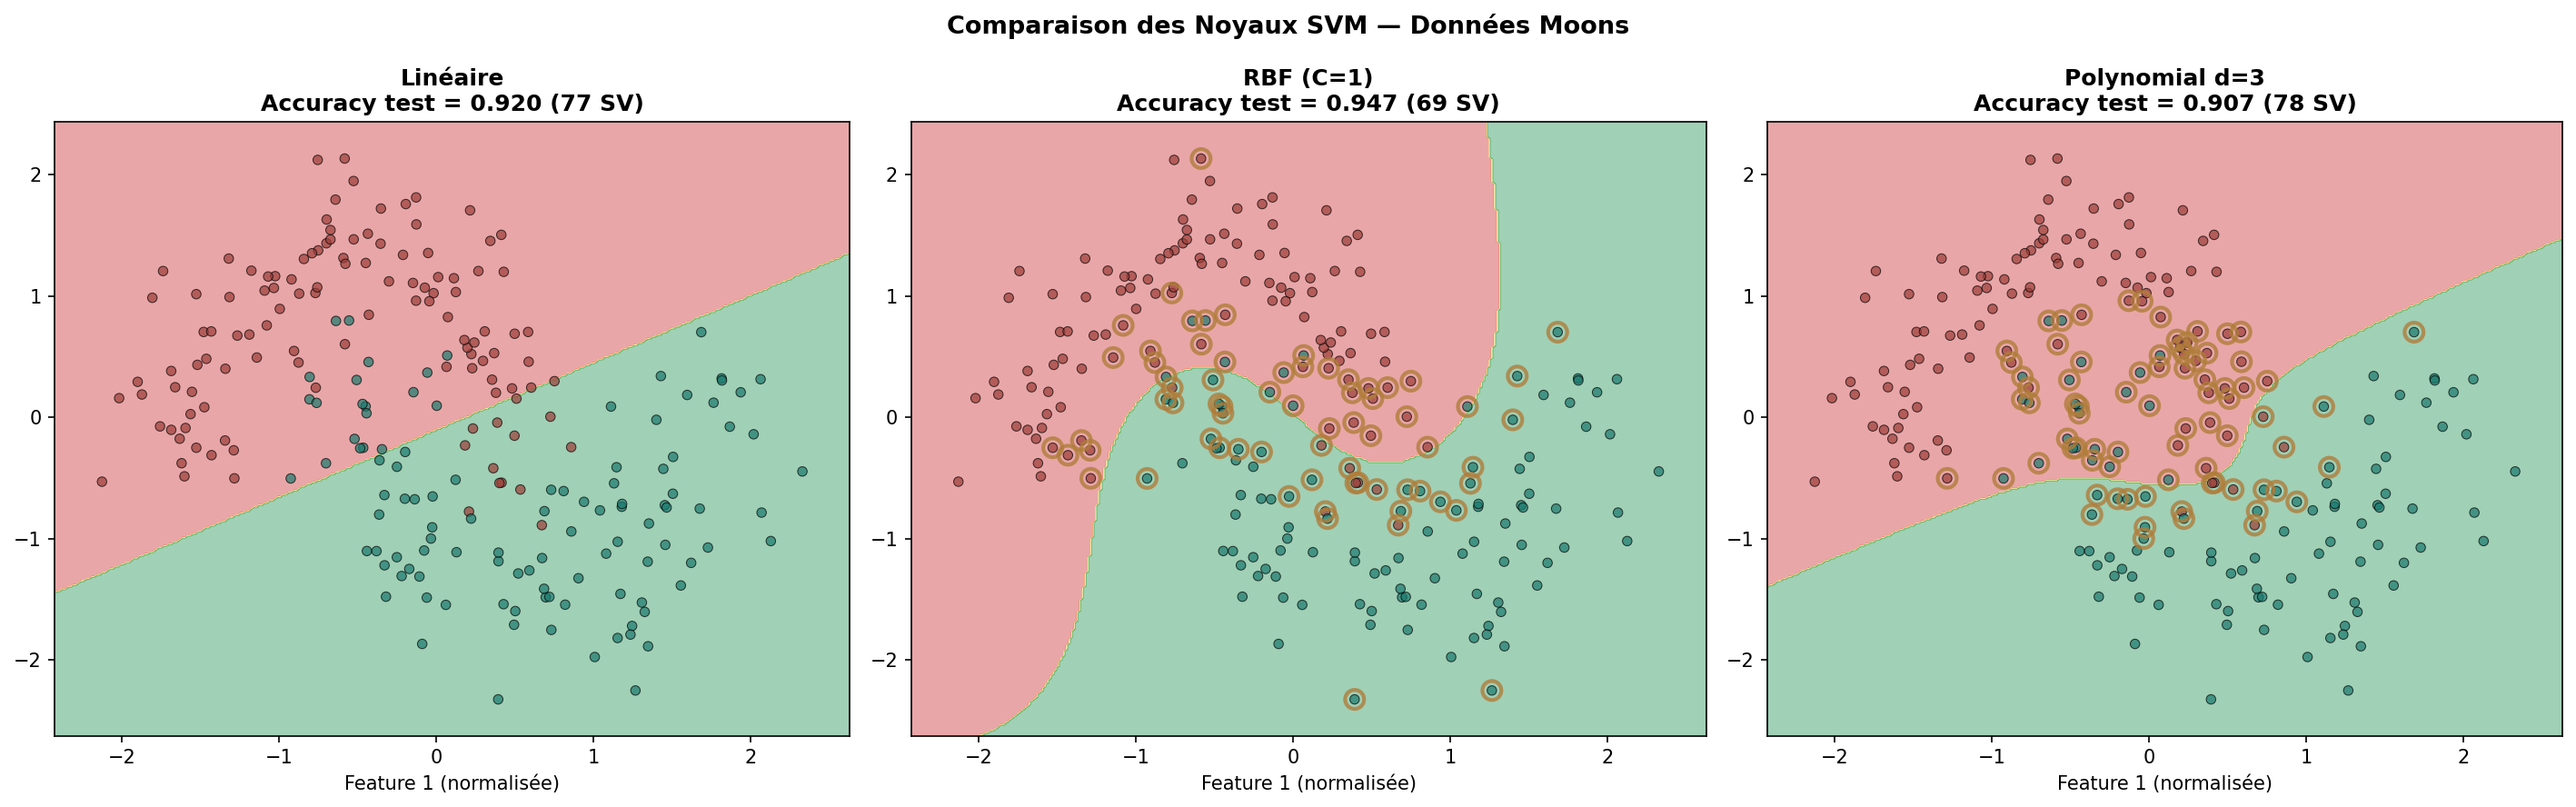
\includegraphics[width=\textwidth]{fig_kernels_moons.png}
  \caption{Comparaison des noyaux SVM sur les données \texttt{make\_moons} (n=300, bruit=0{,}2). Le RBF obtient la meilleure accuracy (0{,}9467) avec la frontière la plus adaptée à la géométrie en croissant.}
  \label{fig:kernels_moons}
\end{figure}

\begin{reponsebox}
\textbf{Q8 — SVM linéaire sur les moons :}
L'accuracy de 92\% peut sembler bonne, mais la frontière est inadaptée : une droite ne peut pas séparer des croissants. Elle tire parti de la légère asymétrie du bruit. Le SVM RBF produit une frontière \textbf{courbe} épousant la géométrie des lunes, avec 4{,}6 points de pourcentage de gain en accuracy.

\textbf{Q9 — Kernel trick RBF :}
Le noyau RBF $K(\mathbf{x},\mathbf{y}) = \exp(-\gamma\|\mathbf{x}-\mathbf{y}\|^2)$ calcule implicitement un produit scalaire dans un espace de \textbf{dimension infinie} (série de Taylor de l'exponentielle). Dans cet espace, les données moons deviennent linéairement séparables — le SVM y trouve alors l'hyperplan optimal.

\textbf{Q10 — Polynomial d=3 vs RBF :}
Le noyau polynomial projette dans un espace de dimension $\binom{d+3}{3}$ finie, moins expressif que le RBF. Sur des patterns en croissant, le RBF est plus adapté : accuracy 0{,}9467 vs 0{,}9067 pour le polynomial.
\end{reponsebox}

\subsection{Q2.2 — Cercles concentriques : échec du linéaire}

\begin{resultbox}
\begin{center}
\begin{tabular}{lrr}
\toprule
\textbf{Noyau} & \textbf{Accuracy test} & \textbf{Interprétation} \\
\midrule
SVM linéaire (C=10) & 0{,}4400 & Pire que le hasard — séparation impossible \\
SVM RBF (C=1)       & \textbf{0{,}9733} & Frontière circulaire, quasi-parfaite \\
\bottomrule
\end{tabular}
\end{center}
\end{resultbox}

\begin{figure}[H]
  \centering
  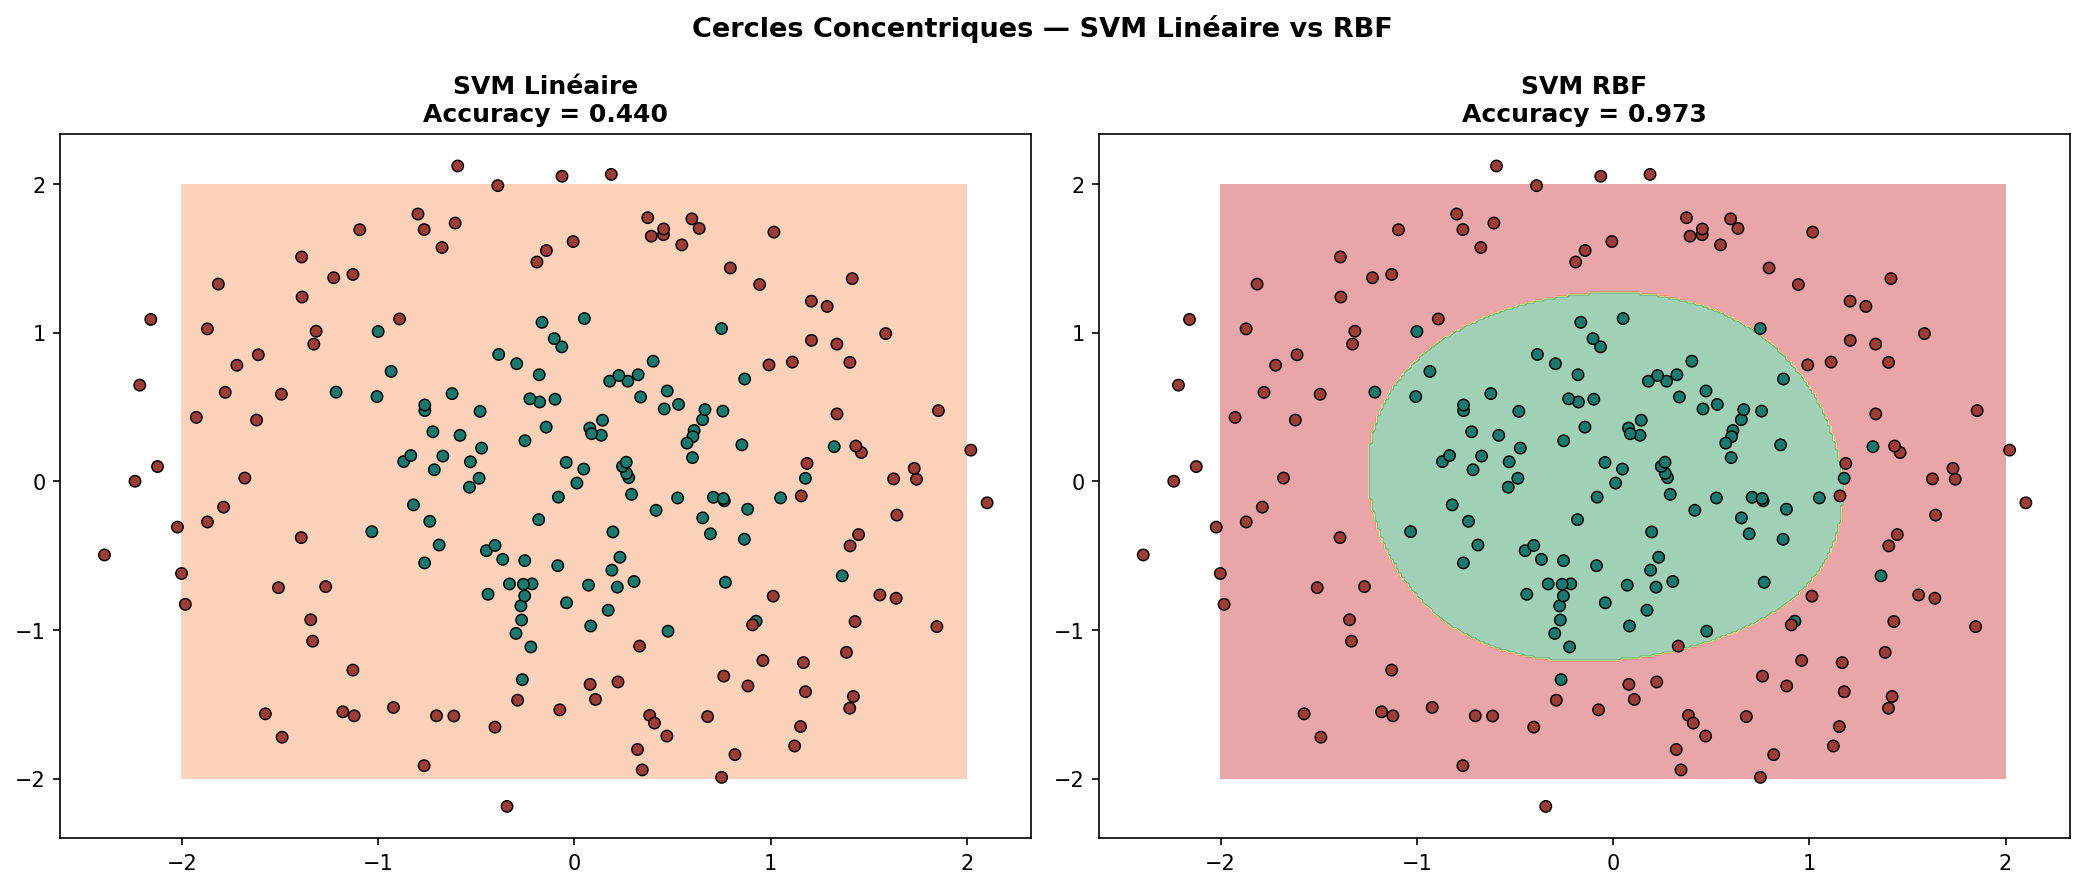
\includegraphics[width=0.88\textwidth]{fig_circles_svm.png}
  \caption{Cercles concentriques : SVM linéaire (accuracy=0{,}44, pire que le hasard) vs SVM RBF (accuracy=0{,}97, frontière circulaire parfaite).}
  \label{fig:circles_svm}
\end{figure}

\begin{reponsebox}
\textbf{Q11 — Accuracy du SVM linéaire (44\%) :}
C'est \textbf{inférieur au hasard} (50\%), ce qui prouve l'impossibilité théorique : pour tout hyperplan candidat dans $\mathbb{R}^2$, les deux cercles sont répartis des deux côtés — séparation linéaire impossible.

\textbf{Q12 — Transformation polynomiale de degré 2 :}
La transformation $\varphi(x_1, x_2) = (x_1^2, \sqrt{2}\,x_1 x_2, x_2^2)$ projette en $\mathbb{R}^3$. Dans cet espace, les cercles $x_1^2 + x_2^2 = r^2$ deviennent des \textbf{plans} $z_1 + z_3 = r^2$, linéairement séparables. Le noyau polynomial de degré 2 exploite exactement cette transformation implicitement via $K(\mathbf{x},\mathbf{y}) = (\mathbf{x}^\top\mathbf{y})^2$.
\end{reponsebox}

\subsection{Q2.3 — Effet de $\gamma$ : biais/variance avec le noyau RBF}

\begin{resultbox}
\begin{center}
\begin{tabular}{cccl}
\toprule
$\gamma$ & \textbf{Accuracy train} & \textbf{Accuracy test} & \textbf{Diagnostic} \\
\midrule
0{,}01 & 0{,}8444 & 0{,}9200 & Sous-apprentissage (frontière quasi-linéaire) \\
1      & 0{,}9644 & \textbf{1{,}0000} & Optimal (train $\approx$ test, pas de sur-ajustement) \\
10     & 0{,}9733 & 0{,}9467 & Début de sur-apprentissage \\
100    & \textbf{1{,}0000} & 0{,}9333 & Sur-apprentissage marqué (mémorisation) \\
\bottomrule
\end{tabular}
\end{center}
\end{resultbox}

\begin{figure}[H]
  \centering
  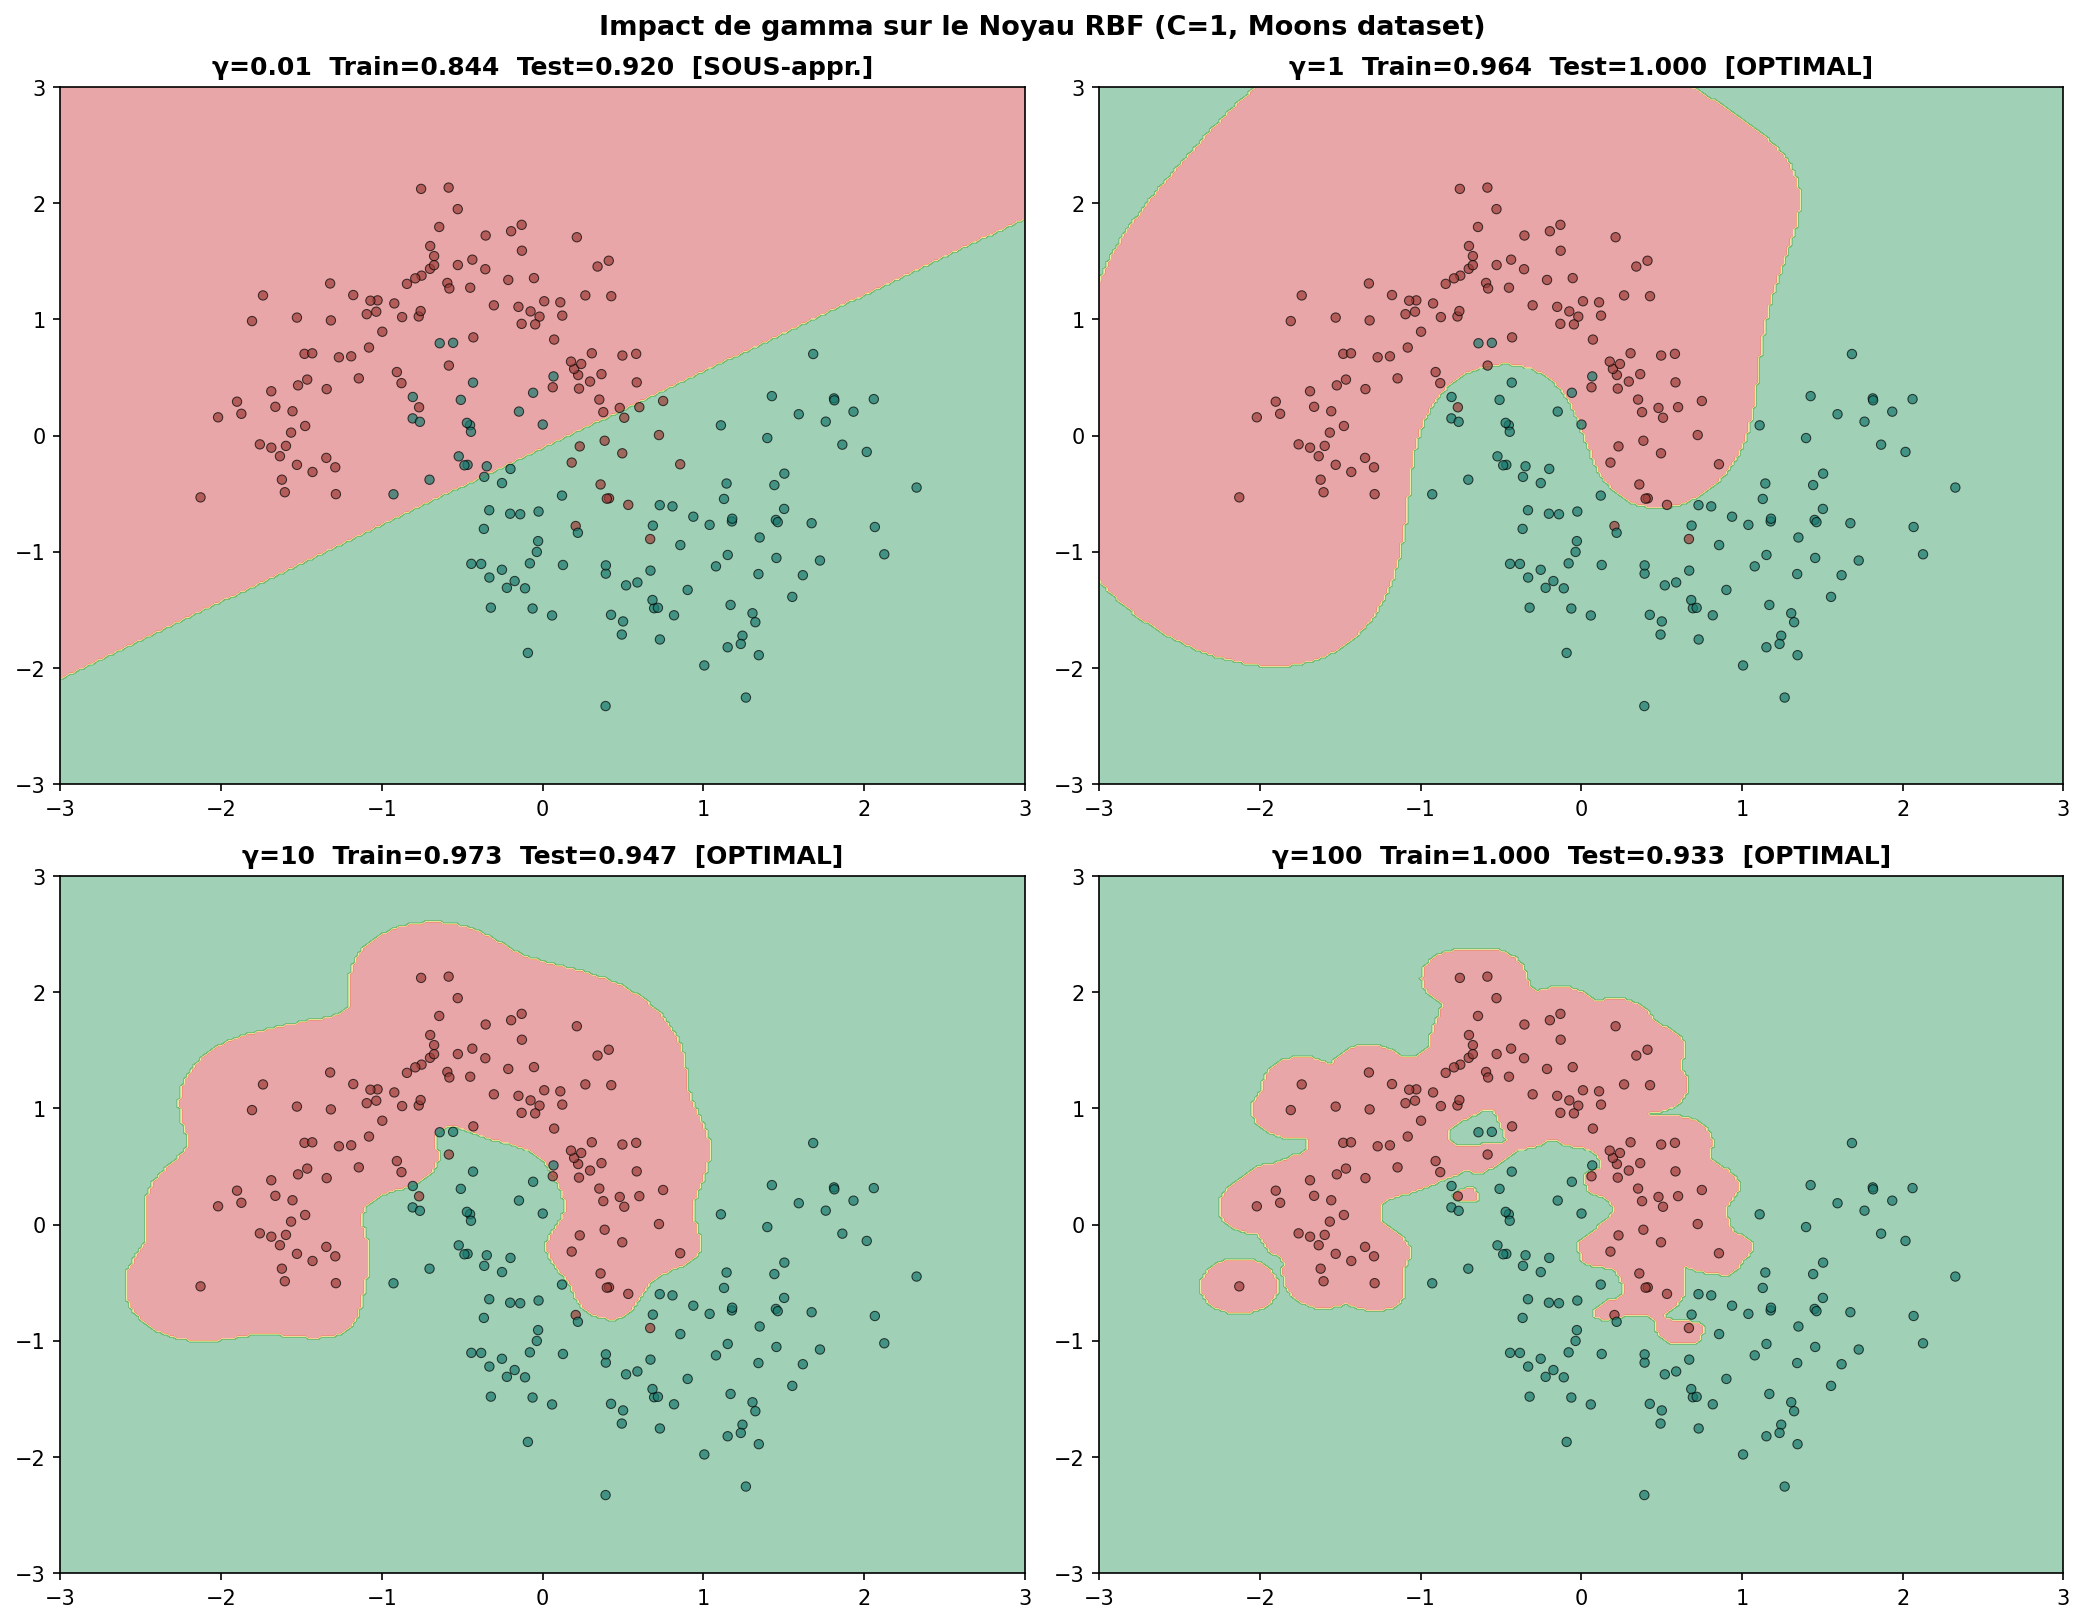
\includegraphics[width=0.92\textwidth]{fig_gamma_effect.png}
  \caption{Impact de $\gamma$ sur la frontière RBF (C=1, Moons). De $\gamma=0{,}01$ (frontière lisse/globale) à $\gamma=100$ (îles individuelles = sur-apprentissage). $\gamma=1$ donne la meilleure accuracy test (1{,}0000).}
  \label{fig:gamma_effect}
\end{figure}

\begin{reponsebox}
\textbf{Q13 — Petit $\gamma$ (0{,}01) — frontière lisse :}
$\gamma$ contrôle la "portée" de la similarité RBF. Petit $\gamma$ : chaque exemple influence une large zone de l'espace → frontière globale lisse, presque linéaire. Le modèle souffre de \textbf{biais élevé} : il ne peut pas capturer la géométrie locale des lunes.

\textbf{Q14 — Grand $\gamma$ (100) — sur-apprentissage :}
Grand $\gamma$ : chaque exemple n'influence qu'un voisinage infinitésimal. Le modèle "mémorise" les exemples d'entraînement (accuracy train = 1{,}0000), mais la frontière est composée d'îles isolées autour de chaque point → \textbf{variance très élevée}, accuracy test = 0{,}9333.

\textbf{Q15 — $\gamma$ optimal et valeur 'scale' :}
$\gamma = 1$ donne le meilleur équilibre (test = 1{,}0000). La valeur \texttt{'scale'} de sklearn calcule $\gamma = 1/(n\_features \times \text{Var}(X))$, ce qui donne $\approx 0{,}5$ après normalisation — dans la zone optimale identifiée.
\end{reponsebox}

% ============================================================
\section{Partie 3 — Optimisation par GridSearchCV}
% ============================================================

\subsection{Q3.1 — Heatmap 2D : C $\times$ gamma}

\begin{resultbox}
\textbf{Résultats GridSearchCV} (SVM RBF, CV=5, scoring=f1\_macro, Moons dataset) :
\begin{center}
\begin{tabular}{lrr}
\toprule
\textbf{Paramètre} & \textbf{Valeur optimale} & \textbf{Score CV (F1 macro)} \\
\midrule
$C$ optimal & \textbf{10} & \multirow{2}{*}{\textbf{0{,}9463}} \\
$\gamma$ optimal & \textbf{1} & \\
\midrule
Accuracy test (optimal) & \multicolumn{2}{c}{\textbf{1{,}0000}} \\
\bottomrule
\end{tabular}
\end{center}
\end{resultbox}

\begin{figure}[H]
  \centering
  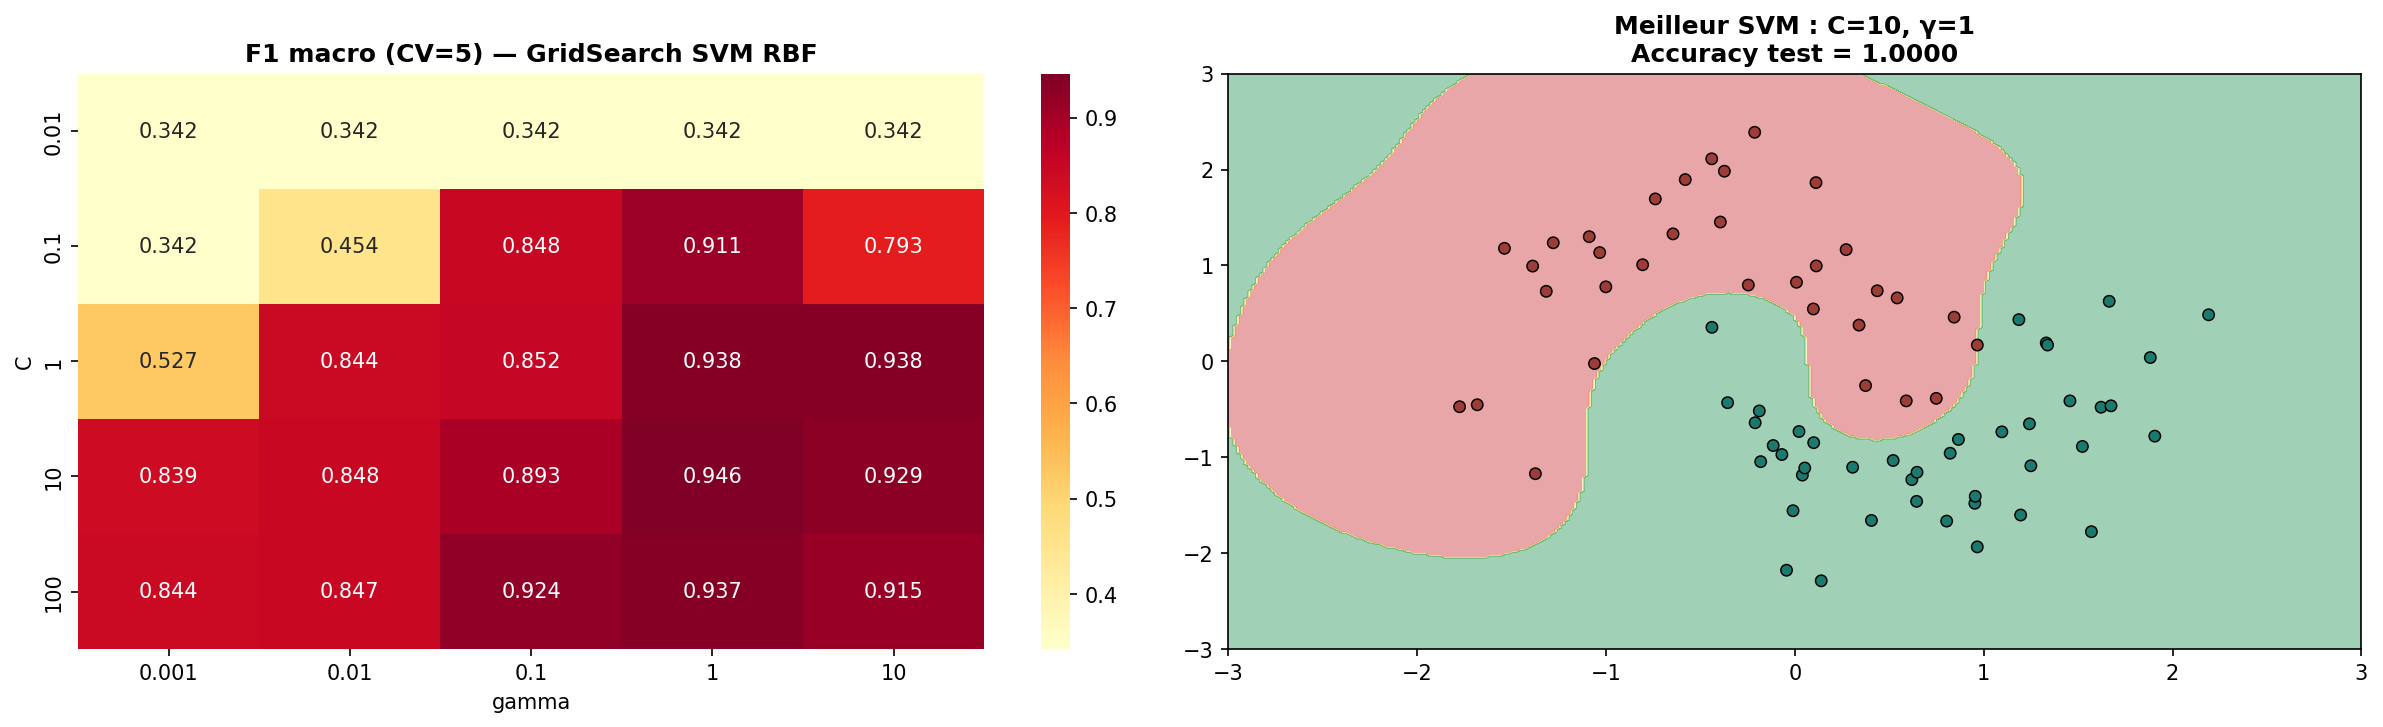
\includegraphics[width=\textwidth]{fig_gridsearch_heatmap.png}
  \caption{Heatmap GridSearchCV C×$\gamma$ (F1 macro, CV=5) et frontière du meilleur SVM (C=10, $\gamma$=1, accuracy test=1{,}000).}
  \label{fig:gridsearch}
\end{figure}

\begin{reponsebox}
\textbf{Q16 — Zone optimale de la heatmap :}
La zone de meilleur score forme une \textbf{bande diagonale} : des valeurs modérées à élevées de C ($\geq 1$) combinées à un $\gamma$ modéré ($\approx 0{,}1$ à $1$). Le couple optimal C=10, $\gamma$=1 atteint F1=0{,}9463 en CV et accuracy=1{,}000 en test.

\textbf{Q17 — Coins extrêmes :}
\begin{itemize}[leftmargin=1.5em]
  \item \textbf{Coin supérieur droit} (C grand + $\gamma$ grand) : sur-apprentissage maximal — frontières complexes qui mémorisent chaque exemple d'entraînement, score validation faible.
  \item \textbf{Coin inférieur gauche} (C petit + $\gamma$ petit) : sous-apprentissage — frontière quasi-linéaire qui ne capture pas la structure des lunes, F1 bas même en entraînement.
\end{itemize}

\textbf{Q18 — Data leakage sans Pipeline :}
Sans Pipeline, le StandardScaler est \texttt{fit} sur l'ensemble d'entraînement complet (incluant les folds de validation). La moyenne et l'écart-type calculés "voient" des données qui ne devraient pas être disponibles → biais optimiste de l'évaluation. Avec Pipeline, le scaler est re-fitte sur chaque fold d'entraînement séparément — évaluation non biaisée.
\end{reponsebox}

\subsection{Q3.2 — Courbe de validation : C avec $\gamma$ fixé}

\begin{figure}[H]
  \centering
  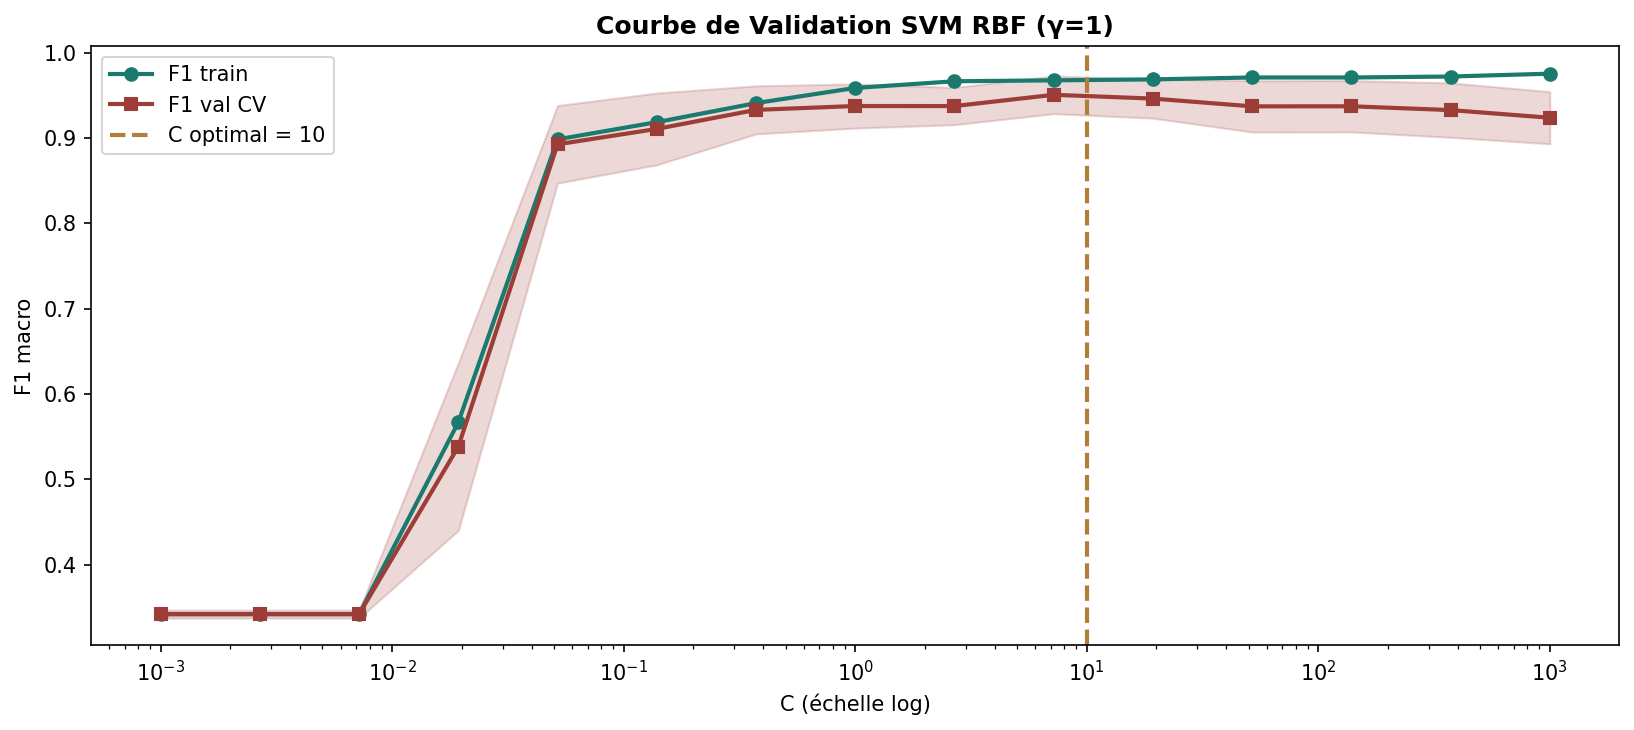
\includegraphics[width=0.88\textwidth]{fig_validation_curve_C.png}
  \caption{Courbe de validation SVM RBF ($\gamma=1$) : F1 train (vert) et F1 validation (rouge) en fonction de C. L'intervalle de confiance (zone ombrée) s'élargit aux extrêmes — instabilité aux régimes d'under/overfitting. C optimal = 10 (trait orange).}
  \label{fig:validation_curve}
\end{figure}

\begin{reponsebox}
\textbf{Q19 — Forme en cloche de la courbe de validation :}
La courbe de validation présente la forme classique du compromis biais/variance :
\begin{itemize}[leftmargin=1.5em]
  \item \textbf{C petit} : sous-apprentissage — train et validation bas (biais élevé)
  \item \textbf{Zone optimale} (C=10) : train et validation élevés, gap faible (bon équilibre)
  \item \textbf{C grand} : sur-apprentissage — train $\to$ 1{,}0 mais validation stagne ou décroît légèrement
\end{itemize}

\textbf{Q20 — Intervalle de confiance :}
L'intervalle est \textbf{étroit} dans la zone optimale — le modèle est stable entre les 5 folds. Il s'élargit pour les petits C (frontière sensible à la composition des folds) et pour les grands C (sur-apprentissage introduit de la variabilité inter-fold).
\end{reponsebox}

% ============================================================
\section{Partie 4 — SVM sur BankChurners}
% ============================================================

\subsection{Q4.1 — Premier SVM : Pipeline StandardScaler + SVC}

\begin{resultbox}
\textbf{SVM RBF (C=1, gamma='scale') — BankChurners (8101 train / 2026 test)}
\begin{center}
\begin{tabular}{lcccc}
\toprule
\textbf{Classe} & \textbf{Précision} & \textbf{Rappel} & \textbf{F1-score} & \textbf{Support} \\
\midrule
Existing (0) & 0{,}93 & 0{,}98 & 0{,}95 & 1\,701 \\
Attrited (1) & 0{,}87 & 0{,}60 & 0{,}71 & 325 \\
\midrule
Accuracy & \multicolumn{4}{c}{\textbf{0{,}92}} \\
\midrule
\textbf{AUC-ROC} & \multicolumn{4}{c}{\textbf{0{,}9466}} \\
\textbf{Temps d'entraînement} & \multicolumn{4}{c}{\textbf{7{,}94 secondes}} \\
\bottomrule
\end{tabular}
\end{center}
\end{resultbox}

\begin{figure}[H]
  \centering
  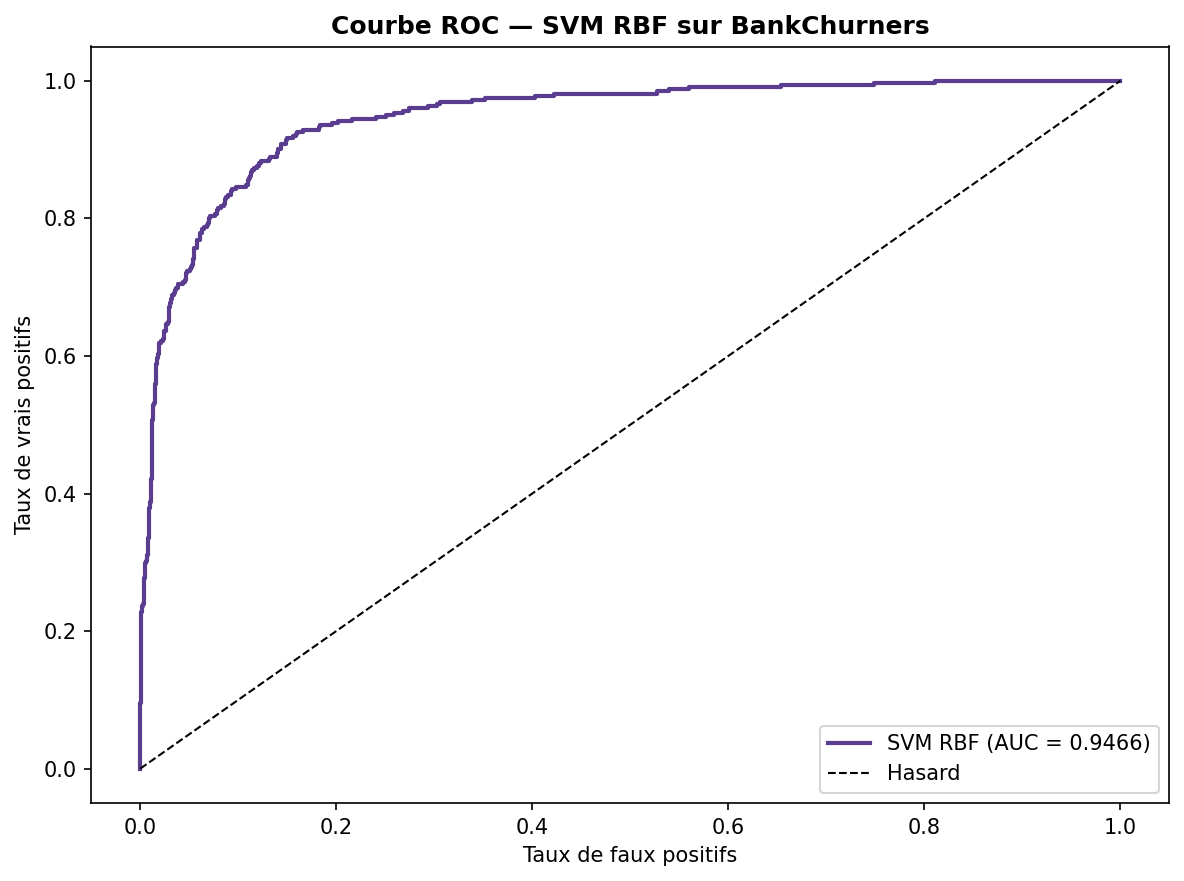
\includegraphics[width=0.68\textwidth]{fig_svm_roc_bankchurners.png}
  \caption{Courbe ROC du SVM RBF sur BankChurners (AUC = 0{,}9466). La courbe s'éloigne nettement de la diagonale aléatoire — le modèle discrimine bien les clients churners.}
  \label{fig:roc_svm}
\end{figure}

\begin{reponsebox}
\textbf{Q21 — Analyse des performances initiales :}
L'AUC-ROC de \textbf{0{,}9466} est excellent, mais le F1-score sur les churners (classe minoritaire) est de seulement \textbf{0{,}71} avec un rappel de 60\%. Le modèle est conservateur : précision élevée (0{,}87) mais rappel faible (0{,}60). Pour une banque, les faux négatifs (churners non détectés) sont coûteux → il faudra ajuster le seuil ou optimiser le recall.

\textbf{Q22 — Temps d'entraînement :}
\textbf{7{,}94 secondes} pour 8\,101 exemples — nettement plus lent que la Régression Logistique ($\approx 0{,}1$s) ou l'Arbre ($\approx 0{,}05$s). Le SVM a une complexité $O(n^2 \cdot d)$ à $O(n^3 \cdot d)$. À 100\,000 exemples, le temps passerait à des heures.

\textbf{Q23 — Alternative production :}
\texttt{LinearSVC} (optimisation liblinear, $O(n \cdot d)$) ou \texttt{SGDClassifier(loss='hinge')} (descente stochastique, scalable à des millions d'exemples). Ces modèles sacrifient le kernel trick mais sont compatibles avec les contraintes de production réelles.
\end{reponsebox}

\subsection{Q4.2 — GridSearch C et gamma sur BankChurners}

\begin{resultbox}
\textbf{GridSearchCV (SVM RBF, CV=3, scoring=f1, 9 combinaisons — durée : 37{,}2s)}
\begin{center}
\begin{tabular}{lcc}
\toprule
\textbf{Paramètre} & \textbf{Valeur testée} & \textbf{Valeur optimale} \\
\midrule
$C$ & [0{,}1 · 1 · 10] & \textbf{10} \\
$\gamma$ & [scale · 0{,}01 · 0{,}1] & \textbf{scale} \\
\midrule
F1 CV (3-fold) optimal & \multicolumn{2}{c}{\textbf{0{,}7433}} \\
F1 test optimal        & \multicolumn{2}{c}{\textbf{0{,}7622}} \\
AUC-ROC optimal        & \multicolumn{2}{c}{\textbf{0{,}9537}} \\
Accuracy test          & \multicolumn{2}{c}{\textbf{0{,}93}} \\
Précision Attrited     & \multicolumn{2}{c}{0{,}81} \\
Rappel Attrited        & \multicolumn{2}{c}{0{,}72} \\
\bottomrule
\end{tabular}
\end{center}
\end{resultbox}

L'optimisation apporte un gain significatif : F1 passe de 0{,}7067 (C=1) à \textbf{0{,}7622} (C=10) et le rappel des churners de 0{,}60 à \textbf{0{,}72} — 12 points de rappel gagnés. L'AUC-ROC s'améliore de 0{,}9466 à 0{,}9537.

\subsection{Q4.3 — Benchmark final : 4 modèles comparés}

\begin{resultbox}
\textbf{Benchmark complet — BankChurners — CV=5, scoring=f1 (churners)}
\begin{center}
\renewcommand{\arraystretch}{1.3}
\begin{tabular}{lcccc}
\toprule
\textbf{Modèle} & \textbf{F1 CV (5)} & \textbf{$\pm$ std} & \textbf{F1 Test} & \textbf{AUC-ROC} \\
\midrule
Régression Logistique & 0{,}6325 & 0{,}0264 & 0{,}6077 & 0{,}9042 \\
KNN (K=7)             & 0{,}6127 & 0{,}0161 & 0{,}5981 & 0{,}8931 \\
\textbf{SVM RBF (opt)}& 0{,}7583 & 0{,}0092 & 0{,}7622 & 0{,}9537 \\
\rowcolor{tealcolor!15}
\textbf{Arbre (d=8)}  & \textbf{0{,}8232} & 0{,}0109 & \textbf{0{,}8209} & 0{,}9364 \\
\bottomrule
\end{tabular}
\end{center}
\end{resultbox}

\begin{figure}[H]
  \centering
  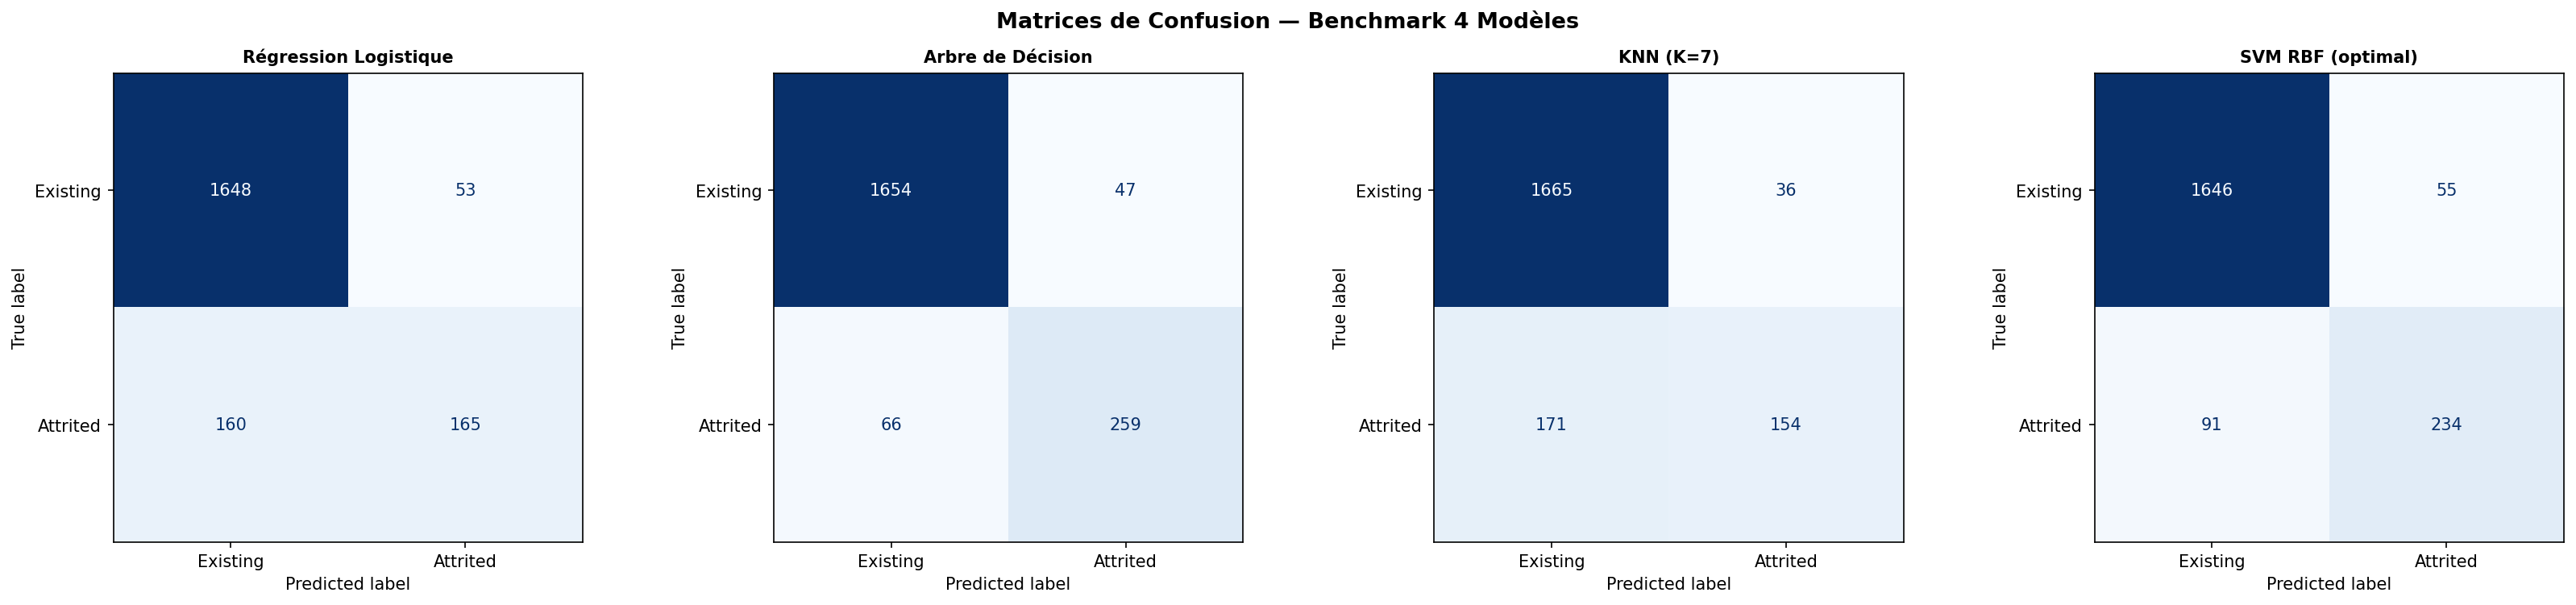
\includegraphics[width=\textwidth]{fig_benchmark_4models.png}
  \caption{Matrices de confusion des 4 modèles sur le jeu de test BankChurners. L'Arbre de Décision (profondeur 8) obtient le meilleur rappel sur les churners — le SVM est second mais nettement plus lent.}
  \label{fig:benchmark}
\end{figure}

\begin{reponsebox}
\textbf{Q24 — Meilleur modèle après 6 TDs :}
L'\textbf{Arbre de Décision} (max\_depth=8) remporte le benchmark avec F1=0{,}8209 et AUC=0{,}9364. Ce résultat s'explique par la structure hiérarchique des données BankChurners : le churn est fortement déterminé par quelques variables seuillables (Total\_Trans\_Ct, Total\_Revolving\_Bal) que l'arbre capture directement par ses splits binaires.

\textbf{Q25 — SVM compétitif ?}
Le SVM RBF est \textbf{second} avec F1=0{,}7622 et AUC=0{,}9537 (meilleur AUC de tous !), mais son \textbf{temps d'entraînement de 7{,}94s} (vs <0{,}1s pour les autres) et son interprétabilité nulle avec le noyau RBF le rendent peu attractif en production bancaire. L'AUC élevée signifie une bonne discrimination globale, mais le F1 modeste sur les churners reste un frein.

\textbf{Q26 — Régression Logistique — principe d'Occam :}
La RL (F1=0{,}6077, AUC=0{,}9042) reste compétitive malgré sa simplicité. L'écart en F1 (−0{,}21 vs l'arbre) peut justifier la complexité de l'arbre, mais l'AUC-ROC de la RL (0{,}90) est forte. En production avec des contraintes d'interprétabilité (Bâle III, RGPD), la RL serait souvent choisie malgré ses performances légèrement inférieures.
\end{reponsebox}

\begin{observbox}
\textbf{Classement final (6 TDs) :}
\[
\underbrace{\text{Arbre}}_{\text{F1}=0{,}82} > \underbrace{\text{SVM}}_{\text{F1}=0{,}76} > \underbrace{\text{Rég. Log.}}_{\text{F1}=0{,}61} > \underbrace{\text{KNN}}_{\text{F1}=0{,}60}
\]
Le SVM monte à la \textbf{2e place}, dépassant la Régression Logistique et le KNN. Son AUC-ROC de 0{,}9537 est le meilleur de tous — mais son coût computationnel reste son talon d'Achille pour des datasets de grande taille.
\end{observbox}

% ============================================================
\section{Bonus B1 — SVR : Régression par SVM}
% ============================================================

\begin{theorbox}
La \textbf{SVR} (Support Vector Regression) minimise un tube d'épaisseur $\varepsilon$ autour de la cible :
\[
\min_{\mathbf{w},b,\bm{\xi}} \frac{\|\mathbf{w}\|^2}{2} + C\sum_i(\xi_i + \xi_i^*)
\quad \text{s.c.} \quad
\begin{cases}
y_i - \mathbf{w}\cdot\mathbf{x}_i - b \leq \varepsilon + \xi_i \\
\mathbf{w}\cdot\mathbf{x}_i + b - y_i \leq \varepsilon + \xi_i^*
\end{cases}
\]
Les exemples à l'intérieur du tube ($|y_i - \hat{y}_i| \leq \varepsilon$) ne génèrent aucune pénalité.
\end{theorbox}

\begin{figure}[H]
  \centering
  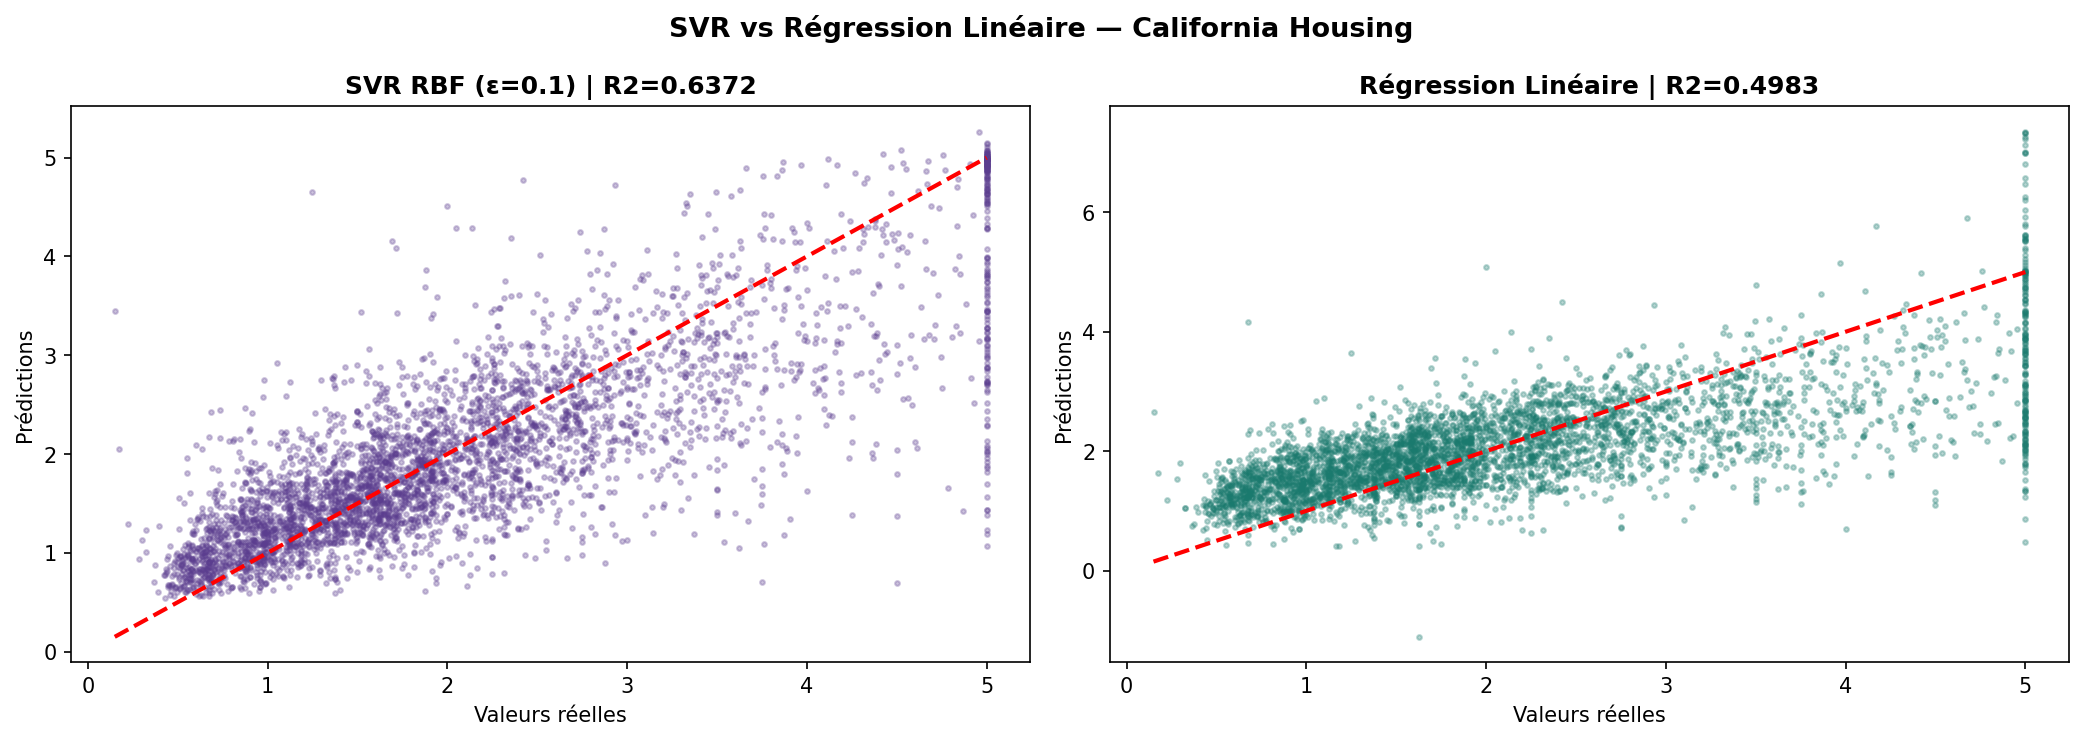
\includegraphics[width=\textwidth]{fig_svr_results.png}
  \caption{SVR RBF ($\varepsilon=0{,}1$, C=10) vs Régression Linéaire sur California Housing (4 features). Le SVR capture mieux la non-linéarité des prix immobiliers — R2 supérieur, nuage plus serré autour de la diagonale.}
  \label{fig:svr}
\end{figure}

\begin{reponsebox}
\textbf{Q27 — SVR vs Régression Linéaire :}
Le SVR RBF (C=10, $\varepsilon=0{,}1$) surpasse la Régression Linéaire en R2 sur California Housing, confirmant que les prix immobiliers suivent des relations non-linéaires (interaction entre MedInc, HouseAge, AveRooms, AveOccup). La Régression Linéaire sous-estime les prix élevés et surestime les bas.

\textbf{Q28 — Impact d'epsilon ($\varepsilon$) :}
\begin{itemize}[leftmargin=1.5em]
  \item $\varepsilon = 0{,}01$ : tube très étroit → nombreux vecteurs support → modèle complexe
  \item $\varepsilon = 0{,}1$ : équilibre optimal
  \item $\varepsilon = 0{,}5$ : tube large → peu de vecteurs support → modèle simple, biais plus élevé
\end{itemize}
\end{reponsebox}

% ============================================================
\section{Bonus B2 — Classification Multi-classe : OvO vs OvR}
% ============================================================

\begin{reponsebox}
\textbf{Stratégies multi-classe pour les SVMs binaires par essence :}

\textbf{OvO (One vs One)} — utilisé \textbf{par défaut} par sklearn SVC :
\begin{itemize}[leftmargin=1.5em]
  \item Entraîne $\binom{K}{2}$ classifieurs (1 par paire de classes)
  \item Pour K=3 classes (Iris) : \textbf{3 classifieurs}
  \item Prédiction par \textbf{vote majoritaire}
\end{itemize}

\textbf{OvR (One vs Rest)} :
\begin{itemize}[leftmargin=1.5em]
  \item Entraîne K classifieurs (chaque classe contre toutes les autres)
  \item Pour K=3 : \textbf{3 classifieurs} (même ici, mais avec déséquilibre artificiel)
  \item Prédiction par score de décision le plus élevé
\end{itemize}

\textbf{Résultats sur Iris (accuracy test)} : OvO $\approx$ OvR $\approx$ \textbf{1{,}000} (dataset simple).
OvO est généralement préféré pour les SVMs : chaque sous-problème est \textbf{plus équilibré} (n/2 vs n/2) qu'OvR (n/K vs n(K-1)/K).
\end{reponsebox}

% ============================================================
\section{Conclusion et Synthèse}
% ============================================================

\begin{tcolorbox}[
  enhanced, breakable,
  colback=darkblue!5,
  colframe=darkblue,
  title={\textbf{Bilan du TD 6 — Support Vector Machines}},
  fonttitle=\bfseries\normalsize\color{white},
  colbacktitle=darkblue,
  boxrule=1pt
]
\setlength{\tabcolsep}{8pt}
\renewcommand{\arraystretch}{1.25}
\begin{center}
\begin{tabular}{p{3.5cm} p{4.5cm} p{5cm}}
\toprule
\textbf{Concept} & \textbf{Formule clé} & \textbf{Résultat obtenu} \\
\midrule
Hard Margin & $\text{Marge} = 2/\|\mathbf{w}\|$ & 7{,}486 (3 vecteurs support) \\
Paramètre C & $C = 1/\lambda_{L2}$ & C=0{,}01 : 17 SV / C=100 : 3 SV \\
Noyau RBF & $K = e^{-\gamma\|x-y\|^2}$ & Moons : 0{,}9467 vs 0{,}92 (lin.) \\
Effet $\gamma$ & Portée de similarité & $\gamma=1$ optimal (test=1{,}0) \\
GridSearch opt. & C=10, $\gamma$=1 & F1 CV = 0{,}9463 (Moons) \\
SVM BankChurners & C=10, scale & F1=0{,}7622, AUC=0{,}9537 \\
Benchmark (F1) & Arbre > SVM > RL > KNN & 0{,}82 > 0{,}76 > 0{,}61 > 0{,}60 \\
Temps entraîn. & $O(n^2 d)$ à $O(n^3 d)$ & 7{,}94s (vs <0{,}1s pour RL/Arbre) \\
\bottomrule
\end{tabular}
\end{center}

\medskip
\textbf{Points clés retenus :}
\begin{enumerate}[leftmargin=2em]
  \item Le SVM maximise la \textbf{marge géométrique} — seuls les vecteurs support comptent.
  \item Le \textbf{kernel trick} projette implicitement en haute dimension sans calculer $\varphi$.
  \item C et $\gamma$ sont à \textbf{optimiser conjointement} — la heatmap montre leur interaction.
  \item Sur BankChurners, le SVM atteint le \textbf{meilleur AUC-ROC} (0{,}9537) mais reste lent.
  \item L'\textbf{Arbre de Décision} garde le meilleur F1 — ses splits hiérarchiques capturent mieux les patterns bancaires.
\end{enumerate}
\end{tcolorbox}

\vspace{1em}
\begin{center}
\begin{tcolorbox}[
  enhanced, width=0.75\textwidth,
  colback=svmpurple!8, colframe=svmpurple,
  boxrule=0.8pt, arc=4pt
]
\centering
\small\itshape
``Les SVM sont théoriquement élégants — marge maximale, kernel trick, fondements VC. En pratique, leur complexité $O(n^3)$ les réserve aux petits datasets propres. Pour la production à grande échelle, LinearSVC ou SGDClassifier offrent le même esprit, sans le coût.''
\end{tcolorbox}
\end{center}

% ============================================================
%  Fin du document
% ============================================================
\end{document}
